\documentclass[12pt]{article}

\usepackage[margin=1in]{geometry}
\usepackage{amsmath,amsthm,amssymb}
\usepackage{mathtools}
\usepackage{mathrsfs}
\usepackage{enumitem}
\usepackage{physics}
\usepackage{empheq}
\usepackage{float}
\usepackage{graphicx}
\graphicspath{ {./images/} }

\usepackage{tikz}
\usetikzlibrary{calc,decorations.markings,patterns}

\newcommand{\magsq}[1]{\big|#1\big|^2}
\newcommand{\avg}[1]{\left<#1\right>}
\newcommand{\fullint}{\int_{-\infty}^\infty}
\newcommand{\fullintd}[1]{\fullint\dd#1\:}
\newcommand{\cint}[2]{\int_{#1}^{#2}}
\newcommand{\cintd}[3]{\cint{#1}{#2}\dd#3\:}

\begin{document}

\title{Homework 1}
\author{Sean Ericson \\ Phys 622}
\maketitle

\section*{$0.2.1$ The brachistochrone problem}
\begin{enumerate}[label=(\alph*)]
    \item Let
    \[ \tilde{g} = g\sin\alpha. \]
    Conservation of energy implies 
    \[ \frac{1}{2}mv^2 = -m\tilde{g}y \implies \boxed{v = \sqrt{-2\tilde{g}y}} \]

    \item The passage time is given by
    \begin{align*}
        T &= \int \frac{\dd s}{v} \\
        &= \int_{x_1}^{x_2}\sqrt{\frac{\dd x^2 + \dd y^2}{-2\tilde{g}y}} \\
        &= \int_{x_1}^{x_2}\sqrt{\frac{\dd x^2 + \left(\dv{y}{x} \dd x\right)^2}{-2\tilde{g}y}} \\
        &= \int_{x_1}^{x_2}\dd x \sqrt{\frac{1 + (y')^2}{-2\tilde{g}y}},
    \end{align*}
    where we identify
    \[ L(y, y') = \sqrt{\frac{1 + (y')^2}{-2\tilde{g}y}}. \]
    Now, using the derivative
    \[ \pdv{L}{y'} = \frac{y'}{1 + (y')^2}\sqrt{\frac{1 + (y')^2}{-2\tilde{g}y}}, \]
    we can write out Jaboci's integral:
    \begin{align*}
        C_1 &= y'\pdv{L}{y'} - L \\
        &= \frac{(y')^2}{1 + (y')^2}\sqrt{\frac{1 + (y')^2}{-2\tilde{g}y}} - \sqrt{\frac{1 + (y')^2}{-2\tilde{g}y}} \\
        &= \frac{-1}{1 + (y')^2}\sqrt{\frac{1 + (y')^2}{-2\tilde{g}y}} \\
        &= \frac{-1}{\sqrt{-2\tilde{g}y(1 + (y')^2)}}.
    \end{align*}
    This equation represents an ODE for $y(x)$.

    \item Let $y' = \cot t$ (note that this implies $\dd x/ \dd y = \tan(t)$). Plugging this into the above ODE gives
    \[ -2\tilde{g}y\csc^2(t) = \frac{1}{C_1^2} \implies \boxed{y(t) = -\frac{\sin^2(t)}{2C_1^2\tilde{g}}}, \]
    with time derivative
    \[ \dv{y}{t} = -\frac{\sin(t)\cos(t)}{2C_1^2\tilde{g}} \]
    Now, 
    \[ \dv{x}{t} = \dv{x}{y}\dv{y}{t} = -\tan(t)\frac{\sin(t)\cos(t)}{2C_1^2\tilde{g}} = -\frac{\sin^2(t)}{C_1^2\tilde{g}} \]
    \[ \implies \boxed{x(t) = \frac{\sin(t)\cos(t) - t}{2C_1^2\tilde{g}} + C_2} \]
    Hey, that's a parameterization of a cycloid!

    \item Let $t_1 = 0$. Then $T = t_2$ and we have that
    \[ T = \cot^{-1}(y'_2) \]
    
    \item Let $P_1$ be the origin. The length of the shortest path between $P_1$ and $P_2$ (a straight line) is therefore
    \[ D = \sqrt{x_2^2 + y_2^2} \]

    \item $\pi$ is the ration of a circle's diameter to its circumference. (Sorry, I didn't get part e finished, so this is the only ratio I can offer)
\end{enumerate}


\section*{$0.2.2$ Dido's problem}
The full Lagriangian is
\[ L = \frac{1}{2}(\dot{x}y - \dot{y}x) + \lambda\sqrt{\dot{x}^2 + \dot{y}^2}. \]
We can start by taking some derivatives:
\begin{align*}
    \pdv{L}{x} &= -\frac{1}{2}\dot{y} \\
    \pdv{L}{y} &= \frac{1}{2}\dot{x} \\
    \pdv{L}{\dot{x}} &= \frac{1}{2}y + \lambda\frac{\dot{x}}{\sqrt{\dot{x}^2 + \dot{y}^2}} \\
    \pdv{L}{\dot{y}} &= -\frac{1}{2}x + \lambda\frac{\dot{y}}{\sqrt{\dot{x}^2 + \dot{y}^2}}
\end{align*}
The Euler-Lagrange equation for the $x$-coordinate gives
\[ -\frac{1}{2}\dot{y} = \frac{1}{2}\dot{y} + \lambda \dv{t}\left(\frac{\dot{x}}{\sqrt{\dot{x}^2 + \dot{y}^2}}\right) \]
\[ \implies -\dv{t}y = \lambda \dv{t}\left(\frac{\dot{x}}{\sqrt{\dot{x}^2 + \dot{y}^2}}\right) \] 
\[ \implies y - y_0 = -\frac{\dot{x}}{\sqrt{\dot{x}^2 + \dot{y}^2}} \]
Similarly, the Euler-Lagrange equation for the $y$-coordinate gives
\[ \frac{1}{2}\dot{x} = -\frac{1}{2}\dot{x} + \lambda \dv{t}\left(\frac{\dot{y}}{\sqrt{\dot{x}^2 + \dot{y}^2}}\right) \]
\[ \implies \dv{t}x = \lambda \dv{t}\left(\frac{\dot{y}}{\sqrt{\dot{x}^2 + \dot{y}^2}}\right) \] 
\[ \implies x - x_0 = \frac{\dot{y}}{\sqrt{\dot{x}^2 + \dot{y}^2}} \]
Squaring and adding the previous two results, we see that
\[ (x-x_0)^2 + (y-y_0)^2 = \lambda^2, \]
which is the equation for a circle centered at $(x_0, y_0)$ with radius $\lambda$. Let the origin be at point $O$, with the $x$-axis pointing along the line $\overline{OP}$, as depicted in Figure \ref{fig1}. By symmetry, we can see that 
\begin{figure}[H]
    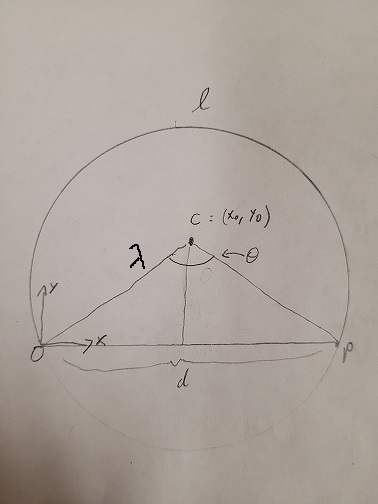
\includegraphics[scale=0.7]{fig1}
    \centering
    \caption{An illustration of the relevent quantities.}
    \label{fig1}
\end{figure}
\[ x_0 = \frac{d}{2}, \]
leaving $y_0$ and $\lambda$ to be determined as a functions of $d$ and $l$. From Figure \ref{fig1}, we can see that
\[ y_0^2 + \left(\frac{d}{2}\right)^2 = \lambda^2, \]
\[ l = (2\pi - \theta)\lambda, \]
and
\[ \sin(\theta/2) = \frac{d}{2\lambda}. \]
These three equations implicitly define $y_0$ and $\lambda$ as functions of $d$ and $l$, but they cannot be solved analytically.



\section*{$0.2.3$ Geodesics on the 2-sphere}
We want to minimize 
\[ \int \dd t \sqrt{\dot{x}^2 + \dot{y}^2 + \dot{z}^2} \]
subject to the constraint
\[ x^2 + y^2 + z^2 = R^2 \]
We start by taking some derivatives. Let 
\[ L_1 = \sqrt{\dot{x}^2 + \dot{y}^2 + \dot{z}^2} \]
then
\[ \pdv{L_1}{\dot{x}} = \frac{\dot{x}}{\sqrt{\dot{x}^2 + \dot{y}^2 + \dot{z}^2}} \]
\[ \pdv{L_1}{\dot{y}} = \frac{\dot{y}}{\sqrt{\dot{x}^2 + \dot{y}^2 + \dot{z}^2}} \]
\[ \pdv{L_1}{\dot{z}} = \frac{\dot{z}}{\sqrt{\dot{x}^2 + \dot{y}^2 + \dot{z}^2}} \]
The Euler-Lagrange equations then give
\[ \dv{t}\frac{\dot{x}}{\sqrt{\dot{x}^2 + \dot{y}^2 + \dot{z}^2}} = 2\lambda x \]
\[ \dv{t}\frac{\dot{y}}{\sqrt{\dot{x}^2 + \dot{y}^2 + \dot{z}^2}} = 2\lambda y \]
\[ \dv{t}\frac{\dot{z}}{\sqrt{\dot{x}^2 + \dot{y}^2 + \dot{z}^2}} = 2\lambda z \]

\end{document}